% !TEX program = xelatex
% 2026-H 车载平衡滚球运动控制系统：竞赛提交版设计报告
% 技术长版保存在同目录下划线前缀文件中，不参与 build.ps1 构建。
% ---- 版式由《2026 年全国大学生电子设计竞赛参赛学生守则》第五条规定，不是可调项 ----
%   正文限 A4 8 页以内 · 首页另附 300 字以内中文摘要 · 正文小四号宋体
%   行距固定值 22 磅 · 每页上方留 3cm 以上空白且空白内不得有任何文字
%   每页右下端注明页码 · 一律 A4 纵向
% 第六条：违反者取消评审、测试资格。原件入库 workbench/参赛守则.jpg。
% 小四 = 12pt；ctexart 默认 \baselineskip = 1.2 x 12pt = 14.4pt，
% 故 \setstretch{1.5278} 得 14.4 x 1.5278 = 22.0pt，即 Word 的“固定值 22 磅”。
\documentclass[12pt,a4paper]{ctexart}

% top 取 3.1cm 而非正好 3.0cm：check_rules.py 量到的是文本块 bbox，含数学符号与表格线
% 的微小上探，正好 3.0cm 时实测最小值为 2.98cm ⇒ 判不合规。0.1cm 余量换确定性。
% ⭐ 守则第五条**只约束上边距**（≥3cm）与纸张/字号/行距，对左右和下边距没有规定。
%   正文 8 页是硬限而内容超了 4 页，所以这里先用掉这块合法空间，再谈删内容：
%   左右 2.4→1.9cm、下 2.2→1.7cm。上边距一分不动。
\usepackage[a4paper,top=3.1cm,bottom=1.7cm,left=1.9cm,right=1.9cm]{geometry}
\usepackage{setspace}
\setstretch{1.5278}
\usepackage{indentfirst}
\setlength{\parindent}{2em}
\setlength{\parskip}{0pt}

\usepackage{amsmath,amssymb,bm}
\usepackage{graphicx}
\usepackage{booktabs,array,multirow}
\newcolumntype{L}[1]{>{\raggedright\arraybackslash}p{#1}}
\renewcommand{\arraystretch}{1.12}
\usepackage{float}
\usepackage{caption}
% 正式图题（“图 N + 文字内容”）采用 9pt 小字；表题保持原来的 small。
\DeclareCaptionFont{figcaption}{\fontsize{9pt}{11pt}\selectfont}
\captionsetup{labelsep=quad}
\captionsetup[figure]{name=图,font=figcaption,skip=6pt}
\captionsetup[table]{name=表,font=small,skip=4pt}
\usepackage{enumitem}
\setlist{nosep,leftmargin=2em}
\usepackage{xcolor}
\usepackage{tikz}
\usetikzlibrary{arrows.meta,positioning,calc}
% ---- 框图视觉编码 ----
% 默认技术图（控制框图、状态机）采用灰阶、线型与线宽，保证黑白打印可辨。
% 整体系统架构图例外：按底盘/滚球/监测三条功能链使用低饱和彩色分区，
% 同时保留链名、空间分区和虚线边界，颜色只帮助建立全局认知，不表示验证状态。
% 验证状态只在图~\ref{fig:hardware} 中登记，避免图的颜色语义随开发进度变化。
\tikzset{
  box/.style={draw,rounded corners=2pt,align=center,minimum height=0.78cm,
              minimum width=2.2cm,font=\small,inner sep=3pt},
  meas/.style={box,fill=black!8},                 % 测量：浅灰底 + 细实线
  ctrl/.style={box,line width=1.1pt},             % 控制：白底 + 粗实线
  act/.style={box,fill=black!20},                 % 执行：深灰底 + 细实线
  mon/.style={box,dashed},                        % 监测：白底 + 虚线（不进控制回路）
  st/.style={box},                                % 状态机常态：白底 + 细实线
  fault/.style={box,dashed,fill=black!14},        % 状态机异常态：虚线 + 灰底
  key/.style={minimum width=0.52cm,minimum height=0.30cm,inner sep=0pt},
  sum/.style={draw,circle,minimum size=0.58cm,inner sep=0pt,font=\small},
  ar/.style={-{Stealth[length=1.8mm]},semithick},
  sgn/.style={font=\scriptsize,inner sep=1pt},
  lbl/.style={font=\scriptsize,inner sep=2pt}
}
\usepackage[hidelinks]{hyperref}

% 页码放右下端（守则第五条）。页眉必须留空——上方 3cm 空白区内不得有任何文字，
% 而 geometry 把页眉放在上边距**之内**，所以只要页眉是空的，那 3cm 就是真空白。
% ⚠️ 刻意不用 fancyhdr：本机 MiKTeX 未装该宏包，赛场断网就装不上。
% 原生 \ps@plain 重定义零依赖，\hfil 把页码顶到文本块右边缘即“右下端”。
\makeatletter
\renewcommand{\ps@plain}{%
  \renewcommand{\@oddhead}{}\renewcommand{\@evenhead}{}%
  \renewcommand{\@oddfoot}{\hfil\thepage}%
  \renewcommand{\@evenfoot}{\hfil\thepage}}
\makeatother
\pagestyle{plain}

\ctexset{
  section/number=\chinese{section},
  section/name={,、},
  section/format=\large\bfseries\raggedright,
  section/beforeskip=0.9ex,
  section/afterskip=0.5ex,
  subsection/number=\arabic{subsection},
  subsection/name={,、},
  subsection/format=\normalsize\bfseries,
  subsection/beforeskip=0.7ex,
  subsection/afterskip=0.3ex
}
\setcounter{tocdepth}{2} % 目录显示到二级标题；三级行题不进目录，避免过密
\setlength{\textfloatsep}{7pt plus 2pt minus 2pt}
\setlength{\floatsep}{6pt plus 2pt minus 2pt}
\setlength{\intextsep}{6pt plus 2pt minus 2pt}
\graphicspath{{figs/}}

\newcommand{\TODO}[1]{{\color{red!80!black}\bfseries[待填：#1]}}
\newcommand{\unit}[1]{\ensuremath{\,\mathrm{#1}}}
% 舵机脉宽单位：全稿只在此处定义，避免 \mathrm{us} 那种错排
\newcommand{\us}{\ensuremath{\,\mu\mathrm{s}}}
\newcommand{\Ohm}{\text{Ω}}
\newcommand{\figplaceholder}[2][0.43\textwidth]{%
  \fbox{\begin{minipage}[c][3.0cm][c]{#1}\centering\color{gray}#2\end{minipage}}}
% 图、表只保留标准 \caption 标题；标题本身即为常规说明，不再另排“简要说明”段落。
% 暂保留空宏以兼容下文既有调用，参数内容不进入 PDF，也不产生额外留白。
\newcommand{\chartnote}[1]{}
% ⚠ 这里曾放过一个「图题器件序号」命令，现已删除（器件名回到图内的引出标注）。
%   两条留给后来人的账，别再重走：
%   ⛔ Unicode ①②③ -> XeLaTeX 派给没有该字形的西文字体，实测 16 个 Missing character，
%      字从 PDF 里静默消失（build.ps1 gate 4c-3 就是为这类缺陷设的）。
%   ⛔ 用 \tikz 现画圈号 -> \tikz 是脆弱命令，放进 \caption 这种移动参数后
%      两个 xelatex 进程双双跑飞（实测 CPU 各烧掉 130~390 秒仍不收敛，只能杀）。

\begin{document}

% =====================================================================
% 封面
\begin{titlepage}
  \centering
  \vspace*{1.5cm}
  {\zihao{2}\bfseries 2026 年全国大学生电子设计竞赛\par}
  \vspace{0.35cm}
  {\zihao{3}\bfseries 赛区赛（TI 杯）设计报告\par}
  \vspace{1.4cm}
  {\zihao{1}\bfseries 车载平衡滚球运动控制系统\par}
  \vspace{0.4cm}
  {\zihao{3}（H 题）\par}
  \vspace{1.5cm}
  \figplaceholder[10cm]{待放：装置整机照片\\（摆杆、相机、循迹阵列与图传发送端均清晰可见）}
  \vspace{1.2cm}
  % 🔴 队员姓名与学校两行已删除, 依据 = 官方《2026 年全国大学生电子设计竞赛参赛学生守则》
  % 第五条原文: "设计封面及每页纸上一律不得出现参赛队学校、队员姓名、代码等文字"; 第六条:
  % "对违反竞赛守则的参赛队, 一经发现, 取消其评审、测试资格"。原模板留着 \TODO{三位队员姓名}
  % 与 \TODO{学校} 两个待填项 ⇒ 照着填就直接违规, 属于"指引本身把人带向取消资格"。
  % 学校/姓名按守则第二条走另附的《登记表》, 不进报告。组别与赛区不在禁列, 保留。
  % 守则原件已入库: workbench/参赛守则.jpg (广东赛区组委会, 2026 年 7 月)。
  {\zihao{4}
  \begin{tabular}{rl}
    组\quad 别： & \TODO{本科组 / 高职高专组} \\[6pt]
    赛\quad 区： & \TODO{赛区} \\[6pt]
    日\quad 期： & 2026 年 8 月 1 日
  \end{tabular}\par}
  \vfill
\end{titlepage}

% =====================================================================
% 摘要
\section*{摘要}
\addcontentsline{toc}{section}{摘要}

% ⚠️ 守则第五条限 300 字，check_rules.py 按 PDF 实际渲染的汉字数计（含 \TODO 占位文字）。
% 三处 \TODO 回填成数字后字数会略降，但增删本节文字前务必重跑 check_rules.py。
针对小车行驶时车体运动扰动钢球的问题，搭建由 MSPM0G3507 完成底盘与滚球控制、固定俯视相机测球位、独立图传供场外观察的车载系统。装机后先用信号发生器测得摆杆机械行程为 $940\sim1340\us$。首轮单侧扫点曾把水平位估为 $1086\us$；闭环四趟平均脉宽以及单变量改中位试验均与之矛盾，故当前改用 $1172\us$，保护窗口内两向余量重算为 $2.81^\circ$ 与 $1.96^\circ$。滚球环现采用位置--速度 PD、轨迹与车体加速度前馈及经验起动补偿；俯仰前馈因对照试验使结果恶化而关闭。底盘低速循迹、球位链路和摆杆输出已有实机数据，监测图传及题目第 1--6 项三轮整机成绩仍待正式验证，不以子系统结果代填。

\noindent\textbf{关键词：}滚球平衡；红外循迹；前馈补偿；姿态测量；机器视觉

\clearpage
\tableofcontents
\clearpage
\pagenumbering{arabic}
\setcounter{page}{1}
\pagestyle{plain}

% =====================================================================
\section{系统方案}

\subsection{任务分析}

题目\cite{q}把六项测试按“监测—底盘—静态滚球—行驶中滚球”逐级叠加，硬指标列于表~\ref{tab:req}。这张表在本报告中只作为验收边界；后文凡未按题目场景完成三轮测试的结果，均不写成对应项目已经达标。

\begin{table}[H]
\centering
\caption{题目要求与验收边界}\label{tab:req}
\small
\setlength{\tabcolsep}{5pt}
\begin{tabular}{cL{7.0cm}L{7.2cm}}
\toprule
项 & 测试场景 & 硬指标 \\
\midrule
1 & 摆杆与钢球位置监测图传 & 场外实时显示，完整录像可现场回放 \\
2 & 从 A 点出发，循迹一圈并停回 A 点 & 时间 $\le20\unit{s}$；停车偏差 $\le2\unit{cm}$ \\
3 & 车静止，钢球由 O 点至 $+5\unit{cm}$，再至 $-5\unit{cm}$ & 总时间 $\le5\unit{s}$；两航点误差均 $\le1\unit{cm}$ \\
4--6 & 载球行驶 AB 或整圈；第 6 项由指定球位起步 & 第 4 项 AB $\le8\unit{s}$；第 5、6 项整圈 $\le30\unit{s}$；球位全程误差 $\le1\unit{cm}$ \\
\bottomrule
\end{tabular}
\end{table}

从测试顺序看，第 2 项可以先单独暴露循迹与停车问题，第 3 项再在车辆静止时检查滚球轨迹；只有第 4--6 项同时叠加车体起停、俯仰和转弯扰动。因此我们没有把整机一次装完后统一调参，而是保留底盘与滚球两条可单独运行的链路。第 1 项图传只供评委观察，按题意不向主控回传数据。

赛道中心线长度为
\begin{equation}
 L=2\times1.5+2\pi\times0.5=6.1416\unit{m}.
\end{equation}
第 2 项 20\unit{s} 门限对应至少 $307.1\unit{mm/s}$ 的平均速度；第 5、6 项 30\unit{s} 门限对应 $204.7\unit{mm/s}$，同时还要求球位全程不超过 $10\unit{mm}$。现有底盘实测却显示，110\unit{RPM} 和 75\unit{RPM} 均会在观察窗内丢线，65\unit{RPM} 才连续运行，按该速度估算一圈约 33\unit{s}。这使“先把巡航速度定高再调滚球”的设想失效：当前先保留能跑稳的低速基线，再用直线快、弯道慢的分段速度争取时间；该分段策略尚未完成正式赛道验证。

第 3 项还给出另一条直接约束：钢球要在 5\unit{s} 内完成 $0\rightarrow+50\rightarrow-50\unit{mm}$，而装机后的摆杆权限只有几度。轨迹时间不能脱离机械行程单独指定。后续先写清实际测到的行程、水平位和对象增益，再说明控制器目前怎样使用这些量；尚未取得的航点误差留到整机三轮测试中判断。

\subsection{三条功能链与总体架构}

调试顺序把系统自然分成三条链。底盘链可在相机与摆杆未投入时独立跑循迹；滚球链可在车架固定时独立辨识和整定；监测链只需把现场画面送到场外。正式测试期间除监测图传外不得与场外设备通信\cite{q}，所以状态估计、任务判断和执行输出均留在车端。

图~\ref{fig:system} 只画已经定义清楚的接口：底盘向滚球侧提供车体速度指令变化和 IMU 姿态，监测链不回传球位或控制指令。图中的颜色用于区分功能，不表示验证状态；各硬件当前证据另见图~\ref{fig:hardware}。

\begin{figure}[H]
\centering
\resizebox{0.98\textwidth}{!}{%
\begin{tikzpicture}[font=\small,
  chain/.style={draw,rounded corners=2pt,align=center,minimum height=0.92cm,
                minimum width=3.2cm,inner sep=4pt},
  drive/.style={chain,fill=green!13,draw=green!45!black},
  ball/.style={chain,fill=blue!10,draw=blue!45!black},
  watch/.style={chain,fill=orange!15,draw=orange!55!black,dashed},
  flow/.style={-{Stealth[length=1.8mm]},semithick},
  watchflow/.style={flow,dashed,draw=orange!65!black},
  lane/.style={font=\small\bfseries,align=right}]
  % 三条水平功能链；颜色之外仍有链名、空间分区与虚线，黑白打印也可读。
  \node[lane,text=green!35!black] at (-2.1,1.8) {底盘运动链};
  \node[drive] (ds) at (0.4,1.8) {八路红外、编码器、IMU\\偏差、里程与姿态};
  \node[drive,line width=0.9pt] (dc) at (5.2,1.8) {循迹、速度与姿态解算\\计时及终点判定};
  \node[drive] (da) at (10.0,1.8) {DRV8231×2、左右电机\\LCD 走时显示};
  \draw[flow] (ds) -- node[above,font=\scriptsize]{状态量} (dc);
  \draw[flow] (dc) -- node[above,font=\scriptsize]{PWM} (da);

  \node[lane,text=blue!45!black] at (-2.1,0) {滚球闭环链};
  \node[ball] (bs) at (0.4,0) {K230 球位相机\\一维球位帧};
  \node[ball,line width=0.9pt] (bc) at (5.2,0) {观测器、PD 与前馈\\轨迹规划及安全限幅};
  \node[ball] (ba) at (10.0,0) {MG995、摇臂拉杆\\摆杆--钢球};
  \draw[flow] (bs) -- node[above,font=\scriptsize]{球位} (bc);
  \draw[flow] (bc) -- node[above,font=\scriptsize]{50 Hz 脉宽} (ba);
  \draw[flow] (ba.south) -- ++(0,-0.55) -| node[below,pos=0.25,font=\scriptsize]{相机反馈} (bs.south);
  \draw[flow] (dc.south) -- node[right,font=\scriptsize,align=left]{$v_{\mathrm{cmd}}\!\to\!\hat a_{\mathrm{veh}}$（启用）\\IMU 俯仰 $\varphi$（补偿关闭）} (bc.north);
  \draw[densely dotted,black!55] (3.25,2.48) rectangle (7.15,-0.68);
  \node[font=\scriptsize,fill=white,inner sep=1.5pt] at (5.2,2.48) {同一 MSPM0G3507 内完成};

  \draw[densely dashed,black!45] (-2.7,-1.05) -- (11.8,-1.05);
  \node[lane,text=orange!55!black] at (-2.1,-2.0) {监测图传链};
  \node[watch] (ws) at (0.4,-2.0) {车载监测相机\\覆盖摆杆全程};
  \node[watch] (wt) at (5.2,-2.0) {图传发送端\\仅共享车载供电};
  \node[watch] (wr) at (10.0,-2.0) {场外接收\\实时显示与录像};
  \draw[watchflow] (ws) -- (wt);
  \draw[watchflow] (wt) -- node[above,font=\scriptsize]{无线视频} (wr);
  \node[font=\scriptsize,text=black!65] at (5.2,-2.75) {本链不向主控回传球位、状态或控制指令};
\end{tikzpicture}}
\caption{车载三条功能链及底盘到滚球控制的定量接口}
\label{fig:system}
\chartnote{绿色、蓝色和橙色分别表示底盘、滚球与监测功能归属；真正连接两个控制问题的是速度指令差分和 IMU 俯仰，监测图传始终在闭环之外。}
\end{figure}

目前这两个接口并非都已定版：速度指令差分前馈保留，俯仰前馈在真机对照中使球位摆幅增大，现已关闭，待姿态零点重新标定后再复测。

\subsection{关键决策记录}

表~\ref{tab:scheme} 不列事后补齐的“完整方案比较”，只保留确实发生过、并改变了实现的三次判断。

\begin{table}[H]
\centering
\caption{由实测结果推动的关键决策}\label{tab:scheme}
\small
\setlength{\tabcolsep}{4pt}
\begin{tabular}{L{1.8cm}L{4.6cm}L{4.2cm}L{4.3cm}}
\toprule
问题 & 观察 & 判断变化 & 当前处理与边界 \\
\midrule
循迹接口 & 串口 FIFO 持续溢出；改接 GPIO 后 93 个样本中八路均响应 & 丢字节发生在硬件取数时限，不在协议解析 & 八路 GPIO + 加权质心；正式一圈待验 \\
摆杆水平位 & 单侧拟合为 $1086\us$；四趟平均输出集中在 $1175\us$ 附近，改中位后偏置降至 $0.5\unit{mm}$ & 单侧样本把零交点拖偏 & 当前取 $1172\us$；待重烧及两侧复测 \\
俯仰前馈 & 全开和只开俯仰均不收敛；静止读数仍约 $-0.7^\circ$ & 姿态零点使补偿本身成为扰动 & 关闭俯仰前馈；重标零点后再复测 \\
\bottomrule
\end{tabular}
\end{table}

% =====================================================================
\section{理论分析与控制设计}

\subsection{循迹速度与可靠性}

八路模块最初按串口接入。实测中接收错误持续增加，进一步按 $115200\unit{baud}$、4 字节 FIFO 核算，主控约每 $348\us$ 就要取数，而 LCD 刷新会使主循环阻塞更久。增加软件缓冲不能补回已经在硬件 FIFO 丢失的字节，因此改为八路 GPIO 同拍读取。改线后手动扫描得到 93 个样本和 35 次位型变化，八路均响应，黑线覆盖通道始终连续；这才把后续整定的反馈基础坐实。

令探头位置为 $p_i\in\{-42,-30,-18,-6,6,18,30,42\}\unit{mm}$，黑线通道记为 $q_i=1$，采用
\begin{equation}
 e_l=\frac{\sum p_iq_i}{\sum q_i},\qquad
 w=\operatorname{sat}\!\left(K_{pl}e_l+K_{dl}\frac{\Delta e_l}{\Delta t},\,\pm w_{\max}\right),
\end{equation}
并令 $v_L=v-w$、$v_R=v+w$。真机移动黑线时，正中读数为 0，最外侧为 $\pm42\unit{mm}$，相邻组合差约 $6\unit{mm}$。装车后还发现 X1 的物理朝向与默认数组相反；先把位置符号改正，再开始调增益，避免把正反馈误判成“参数太大”。

最初的 110\unit{RPM} 巡航在 6.5\unit{s} 丢线，75\unit{RPM} 在 9.4\unit{s} 丢线，65\unit{RPM} 才跑满观察窗。随后保持速度不变，只把 $K_{dl}$ 从 0.05 调到 0.2，偏差摆幅由约 $\pm30$ 收到 $\pm18\unit{mm}$；再加大 $K_{dl}$ 尚无更好证据。当前保留 $K_{pl}=2.0$、$K_{dl}=0.2$、$w_{\max}=70\unit{RPM}$ 和 65\unit{RPM} 低速基线。

一圈按该速度估算超过 $30\unit{s}$，因此程序已加入按 $|w|$ 低通值区分直线和弯道的速度插值。这里没有用 $|e_l|$：实测中偏差大既可能来自弯道，也可能只是一次扰动，不能直接代表曲率。终点采用里程门与启停线联合判定。分段速度和终点判据都已写入程序，但自制赛道当时尚无符合题面尺寸的启停线，故正式一圈结果仍为空。

\subsection{摆杆权限与滚球对象}

装好拉杆后，舵机本体的标称行程已经不能代表机构边界。信号发生器直接驱动实物时，摆杆最低点和最高点分别出现在 $940\us$ 与 $1340\us$；固件据此把保护窗口收在 $960\sim1320\us$。这一步只确认了“能走到哪里”，还没有确认“哪里是水平”。

首轮对象扫点用球加速度对脉宽作线性拟合，得到斜率 $-1.622\,\mathrm{mm\,s^{-2}\,\mu s^{-1}}$ 和零交点 $1086\us$。当时据此把水平位写成 1086\us。闭环试跑随后出现矛盾：无论控制器被告知的中位是 1086 还是 1172\us，四趟稳态平均输出都落在 1158、1186、1188、1192\us；保持其他参数不变，只把中位改为 1172\us，球位均值由 $+11.9$ 变为 $+0.5\unit{mm}$，两向满舵占比也由 0\%/25\% 变为 17\%/17\%。这些现象不能由“1086 是真实水平位”解释，因此当前采用 $1172\us$。首轮扫点只有中位一侧形成了有效运动，零交点受单侧样本拖偏；斜率仍暂作工作区近似，但保留两侧复测要求。

按 $75.4\us/{}^\circ$ 折算，1172\us 到两端保护线的余量分别为 $212\us$ 和 $148\us$，即 $2.81^\circ$ 与 $1.96^\circ$；若要求两个方向都能执行，同一轨迹可依赖的保守权限为 $1.96^\circ$。源码已回填 1172\us，但当前片上版本尚未重烧，试验时用运行时命令设定，报告不把它写成已固化参数。

图~\ref{fig:mechanics} 给出整车纵向布置。$x$ 是钢球相对摆杆中心 $O$ 的位置，$\theta_b$ 是摆杆相对车体的倾角，$\varphi$ 是车体俯仰，$a_{\mathrm{veh}}$ 是车辆纵向加速度。摆杆按题意绕左端合页转动，钢球到合页的距离为 $r=125\unit{mm}+x$。车身长 $290\unit{mm}$，250\unit{mm} 摆杆未伸出车身；支撑台高度和阵列前视距离的实测值仍待补。

% 图必须使用 [H] 嵌在解释段落之后，避免浮到次页而与正文脱节。
% 因此图高需在 TikZ 内控制，不能依赖浮动排版解决。
\begin{figure}[H]
\centering
% scale 0.88（原 0.95）。字号不随 scale 变，缩的是留白不是可读性。
% 相机用图形而不是文字框：文字框在建模图里读起来像流程图节点，不像器件。
\begin{tikzpicture}[scale=0.88,font=\small,
  % 球位相机图标：机身 + 朝下的镜头 + 顶部取景凸起；本图仅绘制进入滚球闭环的相机。
  cam/.pic={
    \draw[semithick,fill=black!8] (-0.34,-0.17) rectangle (0.34,0.17);
    \draw[semithick,fill=black!22] (-0.13,-0.31) rectangle (0.13,-0.17);
    \draw[semithick,fill=black!8] (0.06,0.17) -- (0.12,0.30) -- (0.30,0.30)
      -- (0.30,0.17) -- cycle;
  },
  % 器件名称一律用「引出标注」：文字排在图形四周的空白通道里，细引线指向器件。
  % 这是第四版排法，前三版的账记在这里，别再走回头路：
  %   ① 名称直接贴器件 -> 七个名称互撞，搬一个必撞出另一个（实测三轮）
  %   ② 改带圈数字 -> 不撞了，但要对照图例、观感差（用户否决）
  %   ③ 图题里用 Unicode ①②③ -> 静默缺字 16 处
  %   ④ 现行：名称留在图内（可直接读），但排到外缘通道 -> 既不互撞也不用查表
  lead/.style={gray,line width=0.35pt},
  cl/.style={font=\scriptsize,inner sep=2pt}]
  \coordinate (H) at (0,0);
  \coordinate (E) at (12:6.40);
  \coordinate (O) at (12:3.20);
  \coordinate (B) at (12:4.30);
  % 主图按静止名义姿态绘制：车体平板水平，摆杆相对车体形成 theta_b。
  % 运行时动态俯仰 varphi 不通过倾斜整台车表达，而在平板下方单独画参考线示意。
  % 轮、阵列及尺寸基准均钉在水平平板上，避免把动态扰动误读成装配倾斜。
  % 比例：摆杆 6.40 单位 = 250mm ⇒ 1 单位约 39mm。
  % 2026-07-31 按实车纠正拓扑：
  %   车尾(左) = 支撑台/合页 + 驱动轮；车头(右) = 舵机 + 万向轮；八路阵列在最前端。
  \coordinate (PL) at (-1.0,-0.93);
  \coordinate (PR) at ($(PL)+(0:8.70)$);
  \coordinate (AX) at ($(PL)+(0:2.22)$);   % 驱动轮轴（车尾，与支撑台同侧）
  \coordinate (AR) at ($(PL)+(0:8.45)$);   % 八路阵列（最前端，万向轮之前）
  \coordinate (CS) at ($(PL)+(0:7.70)$);   % 从动万向轮（车头，与舵机同侧）
  \draw[very thick,blue!55!black] (PL) -- (PR);
  \node[cl,anchor=north] (lbplat) at (4.85,-1.06) {车体平板};
  \draw[lead] (lbplat.north) -- (4.85,-0.94);
  \draw[densely dotted,gray] (H) -- ++(0:2.30);
  \node[font=\scriptsize,anchor=north east,fill=white,inner sep=1pt]
    at (1.82,-0.06) {水平基准};
  \draw[-{Stealth[length=1.2mm]}] (0:1.72) arc[start angle=0,end angle=12,radius=1.72];
  \node[font=\scriptsize] at (1.94,0.17) {$\theta_b$};
  % 支撑台 + 合页（摆杆左端）：名称甩到左侧空白通道
  \draw[fill=gray!12] (-0.20,-0.93) rectangle (0.20,-0.04);
  \draw[|<->|,gray] (-0.52,-0.93) -- (-0.52,-0.04)
    node[midway,left,font=\scriptsize,black,inner sep=1.5pt]{$h$};
  \fill (H) circle (2.0pt);
  \node[cl,anchor=east,align=right] (lb1) at (-0.95,-0.30) {支撑台\\与合页};
  \draw[lead] (lb1.east) -- (-0.21,-0.30);
  % 摆杆本体 + 两端防滚落挡片：名称甩到右上空白
  \draw[very thick] (H) -- (E);
  \draw[very thick] (12:0.34) -- ++(102:0.30);
  \draw[very thick] (12:6.25) -- ++(102:0.30);
  \node[cl,anchor=west] (lb8) at (6.42,1.70) {挡片};
  \draw[lead] (lb8.west) -- (6.10,1.58);
  % 钢球、中心点 O、球位 x、铰链到球的距离 r
  \draw[fill=gray!18] (B) circle (0.20);
  % ⚠ 钢球标签由球上方改到球下方：r 尺寸线从球上方掠过，会穿字。
  \node[font=\scriptsize,anchor=north,inner sep=2pt] at ($(B)+(0,-0.26)$) {钢球};
  \fill (O) circle (1.4pt);
  \node[font=\scriptsize,anchor=north,inner sep=2pt] at ($(O)+(-78:0.26)$) {$O$};
  \draw[-{Stealth[length=1.8mm]},semithick]
    ($(O)+(-78:0.64)$) -- ($(B)+(-78:0.64)$)
    node[midway,below,font=\scriptsize,inner sep=1.5pt]{$x$};
  % r 尺寸线向摆杆法向偏移，避开球位相机的视场线。
  \draw[{|[length=1mm]}-{Stealth[length=1.8mm]},semithick,gray]
    ($(H)+(102:0.50)$) -- ($(B)+(102:0.50)$)
    node[pos=0.68,above,font=\scriptsize,black,inner sep=1.5pt]{$r$};
  % 车辆纵向加速度沿水平车体基准，置于平板与摆杆之间的空档。
  \draw[-{Stealth[length=2.0mm]},thick] (3.55,-0.32) -- ++(0:1.35)
    node[midway,above,font=\scriptsize,inner sep=2pt]{$a_{\mathrm{veh}}$};
  % 舵机竖直安装在水平平板上，经摇臂和拉杆抬起摆杆右端。
  \draw[fill=gray!12] (5.02,-0.91) rectangle (5.92,-0.37);
  \node[cl,anchor=west,align=left] (lb3) at (6.22,-0.30) {舵机与\\摇臂拉杆};
  \draw[lead] (lb3.west) -- (5.92,-0.53);
  \coordinate (Hn) at (5.47,-0.37);
  \coordinate (Ht) at (5.82,0.10);
  \fill (Hn) circle (1.2pt);
  \draw[very thick] (Hn) -- (Ht);
  \draw[semithick] (Ht) -- (12:5.90);
  % 动态俯仰只作独立角度定义，不倾斜实际装配主图。
  \coordinate (PHI) at (2.70,-1.63);
  \draw[densely dotted,gray] (PHI) -- ++(0:1.20);
  \draw[densely dashed,gray] (PHI) -- ++(7:1.20);
  \draw[-{Stealth[length=1.0mm]},gray]
    ($(PHI)+(0:0.66)$) arc[start angle=0,end angle=7,radius=0.66];
  \node[font=\scriptsize,anchor=south,fill=white,inner sep=1pt] at (3.30,-1.36)
    {动态俯仰 $\varphi$};
  % ==================== 左右立杆悬挂 + 球位相机 ====================
  % 实物由车身左、右两侧各一根立杆承重，杆顶连接后把相机悬在摆杆正上方；
  % 相机姿态固定、光轴竖直，不随摆杆倾斜。纵向侧视时两杆投影本应重合，
  % 为避免被误读成单杆，图中将远侧杆用虚线横向错开 0.16 单位；这不表示纵向错位。
  % 两杆均从摆杆两侧绕过而不接触，故在摆杆投影交叉处留断口表示遮挡。
  \draw[semithick] (2.12,-0.91) -- (2.12,0.31);
  \draw[semithick] (2.12,0.62) -- (2.12,2.10);
  \draw[semithick,densely dashed] (2.28,-0.91) -- (2.28,0.34);
  \draw[semithick,densely dashed] (2.28,0.65) -- (2.28,2.10);
  \draw[semithick] (2.12,2.10) -- (4.45,2.10);
  \node[cl,anchor=east,fill=white] (lbrods) at (1.35,1.16) {左右立杆};
  \draw[lead] (lbrods.east) -- (2.11,1.16);
  % 球位相机位于钢球运动区正上方，光轴竖直向下，视场收在钢球上。
  \coordinate (CAM) at (4.05,1.76);
  \pic at (CAM) {cam};
  \draw[semithick] ($(CAM)+(0,0.30)$) -- (4.05,2.10);
  \node[cl,anchor=west,align=left] at ($(CAM)+(0.44,0.04)$) {球位相机\\（固定俯视）};
  \draw[dashed,gray] ($(CAM)+(-0.13,-0.31)$) -- ($(B)+(112:0.24)$);
  \draw[dashed,gray] ($(CAM)+(0.13,-0.31)$) -- ($(B)+(64:0.24)$);
  % =============== 整车纵向布置：驱动轮 / 万向轮 / 八路阵列 / 车身界线 ===============
  % 加这一层的理由：式 (3) 的过弯项用了 \ell_p、\S2.1 用了 d_la，而原图既没有驱动轮轴
  % 也没有阵列 ⇒ 两个符号在图上无处可指。同时标出车身长度和摆杆安装范围。
  % 驱动轮（车尾，与支撑台同侧；差速两驱，侧视只见一侧）。
  % 水平平板下两轮取同一触地线 y=-2.03；万向轮较小，悬杆相应缩短。
  \draw[fill=black!12,semithick] ($(AX)+(0,-0.58)$) circle (0.52);
  \fill ($(AX)+(0,-0.58)$) circle (1.4pt);
  \node[cl,anchor=east] (lb2) at (-0.20,-1.55) {驱动轮};
  \draw[lead] (lb2.east) -- ($(AX)+(-0.44,-0.85)$);
  % 从动万向轮（车头，与舵机同侧）。
  \draw[semithick] (CS) -- ($(CS)+(0,-0.80)$);
  \draw[fill=black!6,semithick] ($(CS)+(0,-0.80)$) circle (0.30);
  \node[cl,anchor=east] (lb4) at ($(CS)+(-0.40,-0.80)$) {万向轮};
  \draw[lead] (lb4.east) -- ($(CS)+(-0.31,-0.80)$);
  % 八路循迹阵列位于万向轮之前并贴近同一地面。
  \draw[semithick] (AR) -- ($(AR)+(0,-0.76)$);
  \draw[fill=black!25,semithick]
    ($(AR)+(-0.32,-1.02)$) rectangle ($(AR)+(0.32,-0.76)$);
  \node[cl,anchor=west] (lb5) at ($(AR)+(0.62,-0.89)$) {八路阵列};
  \draw[lead] (lb5.west) -- ($(AR)+(0.33,-0.89)$);
  % ---- 尺寸基准：两条都从驱动轮轴往车头量，与“阵列在转向参考点前方”一致 ----
  % \ell_p 放在平板与摆杆之间，避免增加图的底部高度。
  \draw[densely dotted,gray] ($(AX)+(0,0.10)$) -- (1.21,-0.53);
  \draw[densely dotted,gray] (O) -- (3.13,-0.53);
  \draw[|<->|,gray] (1.21,-0.55) -- (3.13,-0.55)
    node[pos=0.75,fill=white,inner sep=1pt,font=\scriptsize,text=black]{$\ell_p$};
  \draw[densely dotted,gray] ($(AX)+(0,-1.10)$) -- (1.21,-2.16);
  \draw[densely dotted,gray] ($(AR)+(0,-1.02)$) -- (7.42,-2.16);
  \draw[|<->|,gray] (1.21,-2.18) -- (7.42,-2.18)
    node[midway,fill=white,inner sep=1pt,font=\scriptsize,text=black]{$d_{\mathrm{la}}$};
  % 车身纵向界线：题目上限为 350mm，图中按实车长度 290mm 标注。
  % 右端延长线在阵列位置断开，避免穿过阵列方块。
  \draw[densely dotted,gray] (PL) -- (-1.00,-2.50);
  \draw[densely dotted,gray] (PR) -- ($(PR)+(0,-0.40)$);
  \draw[densely dotted,gray] (7.70,-2.36) -- (7.70,-2.50);
  \draw[|<->|,gray] (-1.00,-2.52) -- (7.70,-2.52)
    node[midway,fill=white,inner sep=1pt,font=\scriptsize,text=black]
    {车身长 $290\unit{mm}$，摆杆总长 $250\unit{mm}$（含挡片）};
\end{tikzpicture}
\caption{整车纵向布置与滚球模型坐标（右为车头）}
\label{fig:mechanics}
\chartnote{主图按静止名义姿态绘制：蓝色车体平板水平且 $\varphi=0$，摆杆由支撑台与舵机形成 $\theta_b$；运行时动态俯仰 $\varphi$ 只在平板下方用独立虚线角示意，不表示实际装配倾斜。球位相机由车身左、右两侧立杆悬在摆杆正上方，光轴竖直且不随摆杆倾斜；纵向侧视中将本应重合的两杆略作错开，仅用于表明左右各有一杆。监测图传相机属于独立监测链，本建模图不重复绘制。图中角度与尺寸仅作定义，不可按比例量取。}
\end{figure}

钢球半径 $R_b=5\unit{mm}$，按实心球无滑动滚动处理。由平动、转动方程及 $I=2mR_b^2/5$ 得
\begin{equation}
 \ddot{x}=\frac{5}{7}g\sin\theta=K\sin\theta,
 \qquad K=7007\unit{mm/s^2}.
\label{eq:ball}
\end{equation}
摆杆对地倾角为 $\theta_b+\varphi$。再计入车辆纵向加速度、左端合页构型的离心项和过弯时摆杆中心的向心加速度，可写为
\begin{equation}
 \ddot{x}=\frac{5}{7}\left[g\sin(\theta_b+\varphi)
 -a_{\mathrm{veh}}\cos(\theta_b+\varphi)
 +r\dot\theta_b^{2}-\omega_z^{2}\ell_p\right].
\label{eq:coupled}
\end{equation}
这里的模型用于判断量级，不替代整机测量。按当前机构速度估算，正常跟踪时离心项远小于轨迹加速度；过弯项可能达到毫米级等效偏差，但 $\ell_p$ 尚未实测，所以暂不单独补偿。车辆加速度和俯仰项则直接占用摆角，保留在控制结构中接受真机对照。

首轮扫点在 $1000\us$ 点测得加速度 $+135.1\unit{mm/s^2}$；按斜率外推，$1180\us$ 点应为 $-157.9\unit{mm/s^2}$，与实测相符。因而 $75.4\us/{}^\circ$ 暂作工作区标度，但同一直线的零交点不再采用。

另一次起动试验得到 $0.53^\circ\sim1.59^\circ$ 的分散值。后续位置扫描发现同一脉宽在不同球位既可能保持又可能滚动，说明局部坡度或槽体不直已经混入；当前 $1.20^\circ$ 起动补偿只是经验整定值，不作为纯静摩擦系数。

\subsection{有限摆角下的控制与轨迹}

控制器不是一次按模型定完的。最初按 $\omega_n=3\unit{rad/s}$ 取 $K_p=9$、$K_d=6$，真机却在约 12\unit{mm} 误差时频繁碰到权限边界，球过冲后形成极限环。保持其余量不变，把 $K_p$ 降到 4 后，回中过程变为单调且无过冲；再把 $K_d$ 从 6 加到 9，稳态范围反而由约 $-7.5\sim+15$ 恶化到 $-4.2\sim+22\unit{mm}$，所以退回 6。当前控制律写为
\begin{equation}
 \theta^*=-\frac{K_pe+K_d(\hat v-\dot x_r)+K_i\!\int e\,dt}{K}
 +\frac{\ddot x_r}{K}+I_a\frac{\hat a_{\mathrm{veh}}}{g}
 -I_\varphi\varphi+\theta_f f_s(e),
\label{eq:control}
\end{equation}
其中 $e=\hat x-x_r$，$f_s(e)$ 在目标附近线性回到零。现役值为 $K_p=4\unit{s^{-2}}$、$K_d=6\unit{s^{-1}}$、$\theta_f=1.20^\circ$、$K_i=0$、$I_a=1$、$I_\varphi=0$。$1.20^\circ$ 是两趟静态试跑把范围收进约 $-8.3\sim+10.8\unit{mm}$ 后保留的经验值；由于槽体局部坡度尚未分离，它不被解释为已辨识的库仑摩擦。

俯仰前馈原本按式~\eqref{eq:coupled} 接入，四趟单变量对照却显示：全关时摆幅约 95\unit{mm}，只开车体加速度前馈时末段收敛最好；全开和只开俯仰时摆幅分别约 205\unit{mm} 与 186\unit{mm}，且不收敛。静止读数仍约 $-0.7^\circ$，已足以占用很大一部分权限。因此当前先关闭俯仰补偿，而不是用理论正确性覆盖这组真机反例。弱积分能力虽已写入程序，旧的 $15\unit{mm}$ 偏置在改正水平位后降到 $0.5\unit{mm}$，尚无数据支持默认开启，故 $K_i$ 保持为零。

相机约 24\unit{fps}，滚球环为 50\unit{Hz}，部分控制拍没有新位置。观测器先用上一拍输出和车体运动预测，再以真实帧间隔修正：
\begin{equation}
 \hat x=\hat x^-+\alpha(z-\hat x^-),\qquad
 \hat v=\hat v^-+\frac{\beta}{T_m}(z-\hat x^-).
\end{equation}
$\alpha$ 由 0.5 增至 0.8 时路径误差与过冲同时下降，增至 0.9 又变差，故当前取 $\alpha=0.8$、$\beta=0.5333$。测量超过 150\unit{ms} 未更新时，程序回到水平指令并退出正常控制。该保护链路已实现，整车断开 USB 后 K230 是否仍由车载 5\unit{V} 稳定供电尚待复验。

\begin{figure}[H]
\centering
\begin{tikzpicture}[font=\small]
  \node[box,minimum width=2.5cm]  (ref)   at (0,0)    {轨迹规划\\$x_r,\dot x_r,\ddot x_r$};
  \node[sum]                      (sum1)  at (2.35,0) {$\Sigma$};
  \node[ctrl,minimum width=2.8cm] (pd)    at (4.45,0) {位置--速度 PD\\起动补偿（$K_i=0$）};
  \node[sum]                      (sum2)  at (6.85,0) {$\Sigma$};
  \node[act,minimum width=2.8cm]  (srv)   at (9.05,0) {限幅、舵机与拉杆};
  \node[lbl,anchor=north] at (9.05,-0.48) {$\pm3^\circ$ 上层；$960\sim1320\us$ 硬限};
  \node[box,minimum width=2.3cm]  (plant) at (12.0,0) {摆杆--钢球};
  \node                           (out)   at (14.0,0) {$x$};
  \draw[ar] (ref) -- (sum1);
  \draw[ar] (sum1) -- (pd);
  \draw[ar] (pd) -- (sum2);
  \draw[ar] (sum2) -- (srv);
  \draw[ar] (srv) -- node[lbl,above]{$\theta_b$} (plant);
  \draw[ar] (plant) -- (out);

  \node[box,minimum width=4.6cm] (ff) at (6.85,1.55)
    {当前启用：$\ddot x_r/K+\hat a_{\mathrm{veh}}/g$};
  \node[ctrl,minimum width=2.8cm] (axsrc) at (3.2,2.75) {底盘速度斜坡\\差分得 $\hat a_{\mathrm{veh}}$};
  \node[mon,minimum width=2.5cm] (pitsrc) at (10.3,2.75) {IMU 俯仰 $\varphi$\\补偿当前关闭};
  \draw[ar] (ref.north) -- (0,1.55) -- (ff.west);
  \draw[ar] (axsrc.south) -- (5.2,1.55);
  \draw[ar] (ff) -- (sum2);

  \node[meas,minimum width=2.4cm] (cam) at (11.9,-1.8) {相机约 24\unit{fps}};
  \node[ctrl,minimum width=3.2cm] (obs) at (6.4,-1.8) {$\alpha$--$\beta$ 观测器};
  \draw[ar] (13.7,0) -- (13.7,-1.8) -- (cam.east);
  \draw[ar] (cam.west) -- node[lbl,above]{$z$} (obs.east);
  \draw[ar] (obs.west) -- (2.35,-1.8) -- node[lbl,right,pos=0.55]{$\hat x,\hat v$} (sum1.south);
  \node[sgn] at (2.03,0.20) {$+$};
  \node[sgn] at (2.65,-0.30) {$-$};
  \node[sgn] at (6.53,0.20) {$+$};
  \node[sgn] at (7.04,0.48) {$+$};
\end{tikzpicture}
\caption{滚球控制当前接线；俯仰补偿因真机对照恶化而暂时断开}
\label{fig:ballctrl}
\end{figure}

往返轨迹沿用三角形加速度。出发段 $0\rightarrow+50\unit{mm}$ 取 1.6\unit{s}，返回段 $+50\rightarrow-50\unit{mm}$ 取 2.0\unit{s}，峰值加速度分别为 78.1 与 $100\unit{mm/s^2}$，对应前馈摆角 $0.64^\circ$ 和 $0.82^\circ$；加上 0.2\unit{s} 停留与 1.0\unit{s} 稳定，总规划时间 4.8\unit{s}。这两个角度低于当前保守双向权限 $1.96^\circ$，只说明轨迹在静态权限预算内，不说明航点误差已经满足 $10\unit{mm}$。

滚球层当前限幅为 $\pm3.0^\circ$，目的是保留较大一侧的执行空间；舵机层仍按 $960\sim1320\us$ 对两向作不对称硬裁剪。该做法在一侧发生裁剪时会使观测器使用的指令角与实际角不完全一致，是正式验收前仍需检查的边界。图~\ref{fig:ballparam} 按测量发生的先后给出水平位判断怎样被改写，而不是把当前参数画成一次推导完成的结果。

\begin{figure}[H]
\centering
\resizebox{0.98\textwidth}{!}{%
\begin{tikzpicture}[font=\small,
  pnode/.style={draw,rounded corners=2pt,align=center,minimum height=1.02cm,inner sep=4pt},
  pmeas/.style={pnode,fill=black!10},
  pnow/.style={pnode,line width=1.15pt},
  preject/.style={pnode,dashed,fill=black!3,text=black!65},
  ppending/.style={pnode,dashed},
  parr/.style={-{Stealth[length=1.8mm]},semithick}]
  \node[pmeas,minimum width=4.4cm] (travel) at (-4.4,1.50)
    {信号发生器实测：机械停止点 $940\sim1340\us$};
  \node[pnow,minimum width=3.4cm] (guard) at (1.0,1.50)
    {当前保护窗口：$960\sim1320\us$};
  \draw[parr] (travel) -- (guard);

  \node[preject,minimum width=2.7cm,minimum height=1.28cm] (first) at (-5.85,-0.10)
    {首轮单侧拟合\\零交点 $1086\us$\\后被证据推翻};
  \node[pmeas,minimum width=4.0cm,minimum height=1.38cm] (evidence) at (-2.10,-0.10)
    {四趟均值 $1158/1186/1188/1192\us$\\只改中位：$+11.9\to+0.5\unit{mm}$\\两向满舵：$0/25\%\to17/17\%$};
  \node[pnow,minimum width=2.9cm,minimum height=1.28cm] (center) at (1.55,-0.10)
    {当前水平位 $1172\us$\\源码已回填\\片上待重烧};
  \node[pnow,minimum width=3.9cm,minimum height=1.48cm] (authority) at (5.25,-0.10)
    {两向物理余量\\$212\us=2.81^\circ$\\$148\us=1.96^\circ$\\双向预算 $\pm1.96^\circ$};
  \draw[parr] (first) -- (evidence);
  \draw[parr] (evidence) -- (center);
  \draw[parr] (center) -- (authority);
  \draw[parr] (guard.east) -- ++(0.35,0) |- (authority.north);

  \node[ppending,minimum width=6.5cm,minimum height=0.96cm] (traj) at (3.85,-1.85)
    {现役轨迹 $1.6/0.2/2.0/1.0\unit{s}$；前馈峰值 $0.82^\circ$\\正式航点误差待三轮验证};
  \draw[parr] (authority) -- (traj);
\end{tikzpicture}}
\caption{摆杆水平位由首轮单侧拟合到闭环复核的修正过程}
\label{fig:ballparam}
\end{figure}

% =====================================================================
\section{电路与程序设计}

\subsection{测量与执行链}

主控采用 MSPM0G3507\cite{mspm0}，两片 DRV8231\cite{drv} 驱动左右电机。电机额定 7.4\unit{V}、母线 12\unit{V}，PWM 上限设为 60\%；编码器在 5\unit{kHz} 节拍中作四倍频解码。单路功率与电流采样电路见图~\ref{fig:driver}。

两次接口问题改变了程序结构。八路循迹串口先在硬件 FIFO 丢字节，改为 GPIO 同拍读取；K230 球位帧仍走 UART，但主循环轮询同样出现溢出，于是改由 5\unit{kHz} 节拍只搬字节进环形缓冲，主循环再解析完整帧。改动前相机无有效帧且错误持续增长，改动后实测约 24\unit{fps}、检测率 100\%，连续观察中错误计数不再增长。控制参数是在这条反馈链稳定之后才继续调整。

\begin{figure}[H]
\centering
\begin{tikzpicture}[font=\small,
  cbox/.style={draw,rounded corners=2pt,align=center,minimum height=0.72cm,
               minimum width=2.5cm,inner sep=3pt},
  ca/.style={-{Stealth[length=1.6mm]},semithick}]
  \node[cbox] (pwm) at (-4.5,0) {MSPM0 PWM};
  \node[cbox,line width=1pt] (drv) at (-1.2,0) {DRV8231};
  \node[cbox] (mot) at (2.1,0) {直流电机};
  \node[cbox,fill=black!7] (adc) at (5.25,0) {IPROPI--680~\Ohm--ADC};
  \draw[ca] (pwm) -- (drv);
  \draw[ca] (drv) -- (mot);
  \draw[ca] (drv.south) -- ++(0,-0.42) -| (adc.south);
  \node[font=\scriptsize,anchor=north] at (-1.2,-0.48) {12\unit{V} 母线；PWM 上限 60\%};
\end{tikzpicture}
\caption{单路电机驱动与电流监测信号流；完整原理图见附录 B}
\label{fig:driver}
\end{figure}

供电按 12\unit{V} 电机母线、5\unit{V} 舵机/视觉、3.3\unit{V} 逻辑三档规划。这里仍有未闭合的实物边界：K230 目前断开 USB 后曾出现球位停止更新，尚需确认改接车载 5\unit{V} 后能冷启动并持续发帧；MG995 换向时 5\unit{V} 最低电压和主控是否复位也未测。图~\ref{fig:hardware} 因而把“已通链路”和“待车载供电复验”分开标出。

\begin{figure}[H]
\centering
\resizebox{0.98\textwidth}{!}{%
\begin{tikzpicture}[font=\small,
  hw/.style={draw,rounded corners=2pt,align=center,minimum height=1.02cm,
             minimum width=3.0cm,inner sep=3pt},
  hmon/.style={hw,dashed},
  hwar/.style={-{Stealth[length=1.7mm]},semithick},
  hmwar/.style={hwar,dashed}]
  \fill[orange!8,rounded corners=3pt] (-7.2,1.92) rectangle (7.2,0.78);
  \fill[blue!7,rounded corners=3pt]   (-7.2,0.57) rectangle (7.2,-0.57);
  \fill[green!8,rounded corners=3pt]  (-7.2,-0.78) rectangle (7.2,-1.92);
  \node[font=\small\bfseries,text=orange!55!black,anchor=west] at (-7.0,1.35) {监测链};
  \node[font=\small\bfseries,text=blue!45!black,anchor=west] at (-7.0,0) {滚球链};
  \node[font=\small\bfseries,text=green!35!black,anchor=west] at (-7.0,-1.35) {底盘链};

  \node[hmon,minimum width=4.1cm] (moncam) at (-3.45,1.35)
    {监测相机 + 树莓派 5\\{\scriptsize 待上电与图传联调}};
  \node[hmon,minimum width=4.1cm] (viewer) at (4.0,1.35)
    {场外浏览器\\{\scriptsize 实时显示、录像待三轮验证}};
  \draw[hmwar] (moncam) -- node[above,font=\scriptsize]{无线视频；不回传控制} (viewer);

  \node[hw,fill=black!7,minimum width=4.1cm] (ballsens) at (-3.45,0)
    {K230 球位（UART，约24\unit{fps}）\\ICM-42688-P 姿态（SPI）\\{\scriptsize 两条信号链已通}};
  \node[hw,line width=1.1pt,minimum width=2.75cm] (ballctrl) at (0.35,0)
    {MSPM0G3507\\滚球观测与控制};
  \node[hw,fill=black!17,minimum width=3.55cm] (ballact) at (4.55,0)
    {MG995 + 摇臂拉杆\\50\unit{Hz} 脉宽\\{\scriptsize 输出链已实测}};
  \draw[hwar] (ballsens) -- (ballctrl);
  \draw[hwar] (ballctrl) -- (ballact);

  \node[hw,fill=black!7,minimum width=4.1cm] (drivesens) at (-3.45,-1.35)
    {八路红外 GPIO + 左右编码器\\{\scriptsize 映射、方向与低速运行已实测}};
  \node[hw,line width=1.1pt,minimum width=2.75cm] (drivectrl) at (0.35,-1.35)
    {同一 MSPM0G3507\\循迹、速度与状态机};
  \node[hw,fill=black!17,minimum width=3.55cm] (driveact) at (4.55,-1.35)
    {DRV8231×2 + 左右电机\\GC9A01 状态与走时\\{\scriptsize 正式一圈待验}};
  \draw[hwar] (drivesens) -- (drivectrl);
  \draw[hwar] (drivectrl) -- (driveact);

  \node[draw,rounded corners=2pt,fill=black!5,align=center,minimum width=14.4cm,
        minimum height=0.64cm] (power) at (0,-2.55)
    {供电：12\unit{V}$\rightarrow$电机；5\unit{V}$\rightarrow$MG995、K230 与监测链（负载跌落待验）；3.3\unit{V}$\rightarrow$主控、传感器与 LCD};
\end{tikzpicture}}
\caption{控制硬件三条泳道与供电边界；括号内为当前实物证据}
\label{fig:hardware}
\end{figure}

球位相机由两侧立杆固定在摆杆上方，不随摆杆转动。相机端已用摆杆两端的已知位置建立像素到毫米映射；视觉端自报 $+96.2\unit{mm}$ 时，主控同期读到 $+97.3\unit{mm}$。这证明串口两端量纲一致，不等于全视场误差已经完成标定。

固定俯视会引入随摆角变化的尺度误差。球心距合页 $r=125\unit{mm}+x$，物距为 $H$ 时，相对误差近似为 $r\sin\theta_b/H$。按当前保守权限 $1.96^\circ$、$x=50\unit{mm}$，球心高度变化约 $6.0\unit{mm}$；$H$、高光偏差及机构回差尚无实测数据，因此暂不把这一项写进已闭合误差预算。

\subsection{任务节拍与失效保护}

程序早期把串口和显示都放在主循环，真实相机接入后出现 FIFO 溢出，才把“搬运”和“解析”拆开：5\unit{kHz} 中断只采编码器、搬 UART 字节；主循环解析帧和刷新显示；IMU、滚球、循迹按各自周期分频。图~\ref{fig:tick} 画的是当前执行层次，不表示各任务计算量相同。

状态机只管理一次测试的起止与失效：IDLE 保持球位，启动后进入 RUN，里程与启停线同时满足才进入 DONE；丢线、视觉超龄、超时或急停进入 ABORT。串口命令已能走通，实体按键和蜂鸣器尚未接线，正式第 2 项流程仍待实物验收。

\begin{figure}[H]
\centering
\begin{tikzpicture}[font=\small]
  \node[st,minimum width=3.0cm,minimum height=0.62cm] (idle) at (0,0) {IDLE（球位保持）};
  \node[st,minimum width=3.8cm,minimum height=0.62cm] (run) at (5.0,0) {\textbf{RUN}（循迹、计时、滚球）};
  \node[st,minimum width=3.0cm,minimum height=0.62cm] (done) at (10.2,0) {DONE（停车、冻结）};
  \node[fault,minimum width=3.5cm,minimum height=0.62cm] (abort) at (5.0,-1.25) {ABORT（停机、显示）};
  \draw[ar] (idle) -- node[lbl,above]{启动} (run);
  \draw[ar] (run) -- node[lbl,above]{里程 + 启停线} (done);
  \draw[ar] (run) -- node[lbl,right]{丢线 / 超龄 / 超时 / 急停} (abort);
\end{tikzpicture}
\caption{主任务状态机；DONE 或 ABORT 复位后回到 IDLE，虚线灰底为异常态}
\label{fig:fsm}
\end{figure}

\begin{figure}[H]
\centering
\begin{tikzpicture}[font=\scriptsize,
  lane/.style={draw,rounded corners=2pt,align=left,text width=13.6cm,
               minimum height=0.62cm,inner xsep=5pt,inner ysep=2pt}]
  \node[lane,fill=black!10] (hard) at (0,0.76)
    {\textbf{硬实时搬运}\quad SysTick 5\unit{kHz}（0.2\unit{ms}）：编码器采样，UART 字节写入环形缓冲};
  \node[lane,fill=black!4] (loop) at (0,0)
    {\textbf{周期控制环}\quad IMU 5\unit{ms}；滚球观测与控制 20\unit{ms}；速度环与循迹 50\unit{ms}};
  \node[lane,fill=black!2] (main) at (0,-0.76)
    {\textbf{低频与主循环}\quad 持续读取环形缓冲、解析完整帧并运行状态机；LCD 走时与状态 100\unit{ms}};
\end{tikzpicture}
\caption{多速率程序的三层调度；中断只搬运，完整帧解析留在主循环}
\label{fig:tick}
\end{figure}

% =====================================================================
\section{测试方案与结果}

\subsection{证据口径与预验证}

正式验收每项做 3 次，以时间、停车偏差和录像中的最大球位偏差与表~\ref{tab:req} 比较；未完成的格保持待填。测试时关闭调试遥测，只保留题目允许的监测图传。

整机测试前已取得以下链路证据：编码器左右轮 10 圈为 952.5、957.0 counts/rev，600\unit{mm} 单趟换算 599.1\unit{mm}；八路循迹共 93 个样本、35 次位型变化，八路均响应且在线通道连续；IMU 的 WHOAMI 为 0x47，静止陀螺 $\le0.42\unit{dps}$，加速度模长 1.009\unit{g}；65\unit{RPM} 低速循迹连续 39.0\unit{s}、累计 7120\unit{mm}，丢线标志为 0。这些数据只确认测量、量纲和低速连续性，不替代第 1--6 项整机成绩。

% ⛔ 这里曾插入 figs/fig_speedloop.pdf 并标注［实测］，已撤除。
% 数据源五列全为零，那一趟车没有运动；不得把空曲线作为实测证据。

\subsection{整机测试结果}

\begin{table}[H]
\centering
\caption{整机三轮原始测试结果；每格按“时间 / 偏差”填写}\label{tab:final}
\small
\setlength{\tabcolsep}{3pt}
\begin{tabular}{cL{4.4cm}cccc}
\toprule
项 & 当轮记录量 & 第 1 次 & 第 2 次 & 第 3 次 & 达标 \\
\midrule
1 & 实时显示；录像回放 & \TODO{} & \TODO{} & \TODO{} & \TODO{} \\
2 & 一圈时间；停车偏差 & \TODO{} & \TODO{} & \TODO{} & \TODO{} \\
3 & 总时间；$\pm5\unit{cm}$ 两端误差 & \TODO{} & \TODO{} & \TODO{} & \TODO{} \\
4 & AB 时间；最大球位误差 & \TODO{} & \TODO{} & \TODO{} & \TODO{} \\
5 & 整圈时间；最大球位误差 & \TODO{} & \TODO{} & \TODO{} & \TODO{} \\
6 & 整圈时间；最大球位误差 & \TODO{} & \TODO{} & \TODO{} & \TODO{} \\
\bottomrule
\end{tabular}
\end{table}

\noindent 第 2 项画面需包含停车位置与 A 点基准线，第 3--6 项需包含球心、目标刻度和时间；第 1 项三轮均须实时显示并能现场回放。未取得影像前，不以示意图代替证据。

\subsection{结果分析}

表~\ref{tab:final} 仍空，以下不是整机结论。\textbf{水平位：}$1086\us$ 被四趟输出和单变量试验推翻；改用 1172\us 后，均值由 $+11.9$ 降至 $+0.5\unit{mm}$，两向满舵由 0\%/25\% 变为 17\%/17\%，故 $K_i=0$。\textbf{起动补偿：}$0.53^\circ\sim1.59^\circ$ 混入局部坡度和槽体不直，$1.20^\circ$ 只因两趟静态结果约为 $\pm10\unit{mm}$ 而暂留。\textbf{轨迹权限：}两向余量 $2.81^\circ/1.96^\circ$ 大于前馈峰值 $0.64^\circ/0.82^\circ$；但上层 $\pm3^\circ$ 与不对称裁剪尚未统一，三轮航点误差也未取得，不能判第 3 项达标。

% =====================================================================
\section{结论}

现有证据只支持继续整机验证。1172\us 尚待重烧，车载供电、5\unit{V} 跌落、俯视误差、机构回差、实体按键、图传及表~\ref{tab:final} 三轮成绩均未验收；结论按最不利值填写：\TODO{结论}。

\clearpage
% =====================================================================
\begin{thebibliography}{9}
\addcontentsline{toc}{section}{参考文献}
\small
\bibitem{q} 全国大学生电子设计竞赛组委会. 2026 年全国大学生电子设计竞赛赛区赛（TI 杯）H 题：车载平衡滚球运动控制系统[Z]. 2026.
\bibitem{mspm0} Texas Instruments. MSPM0G3507 Mixed-Signal Microcontrollers Datasheet (SLASEZ1)[Z]. 2024.
\bibitem{drv} Texas Instruments. DRV8231 Brushed DC Motor Driver Datasheet[Z]. 2023.
\bibitem{icm} TDK InvenSense. ICM-42688-P 6-Axis MotionTracking Device Datasheet[Z]. 2023.
\bibitem{mahony} Mahony R, Hamel T, Pflimlin J M. Nonlinear Complementary Filters on the Special Orthogonal Group[J]. IEEE Transactions on Automatic Control, 2008, 53(5): 1203--1218.
\bibitem{bar} Bar-Shalom Y, Li X R, Kirubarajan T. Estimation with Applications to Tracking and Navigation[M]. Wiley, 2001.
\end{thebibliography}

\clearpage
% =====================================================================
\appendix
\section*{附录 A\quad 电源电路原理图}
\addcontentsline{toc}{section}{附录 A\quad 电源电路原理图}
\begin{figure}[H]
\centering
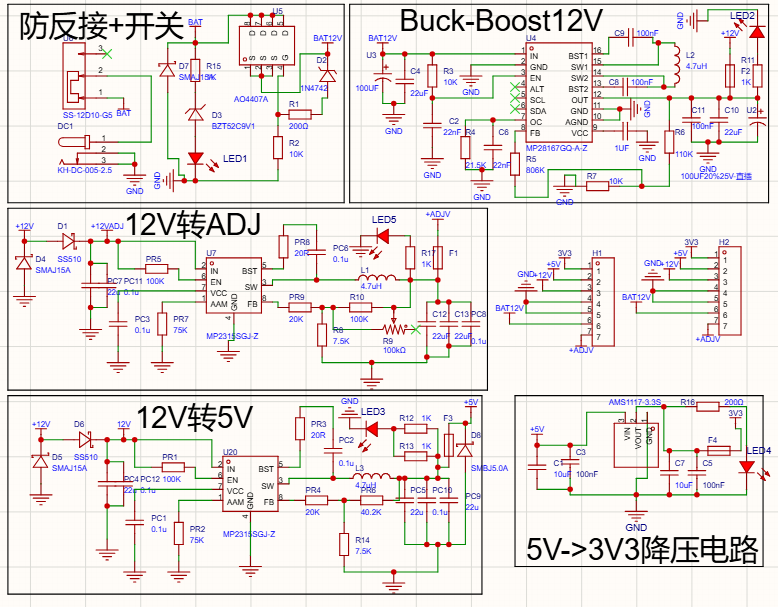
\includegraphics[width=0.96\textwidth]{sch_power}
\caption{自制多路电源板：防反接与总开关、12\unit{V} Buck--Boost 母线、5\unit{V} 与 3.3\unit{V} 支路}
\chartnote{电机、舵机/视觉和逻辑负载分轨供电；当前仍需用舵机换向负载阶跃验证 5\unit{V} 跌落和 3.3\unit{V} 纹波，原理图不能替代该项实测。}
\end{figure}

\noindent 电机驱动接 12\unit{V} 母线；舵机、视觉模块与图传发送端接 5\unit{V}；主控、IMU、循迹阵列和 LCD 接 3.3\unit{V}。舵机与视觉模块定版后，应复测 5\unit{V} 支路负载阶跃以及 3.3\unit{V} 纹波，确认执行器动作不引起主控复位或视觉丢帧。

\clearpage
\section*{附录 B\quad 电机驱动原理图}
\addcontentsline{toc}{section}{附录 B\quad 电机驱动原理图}
\begin{figure}[H]
\centering
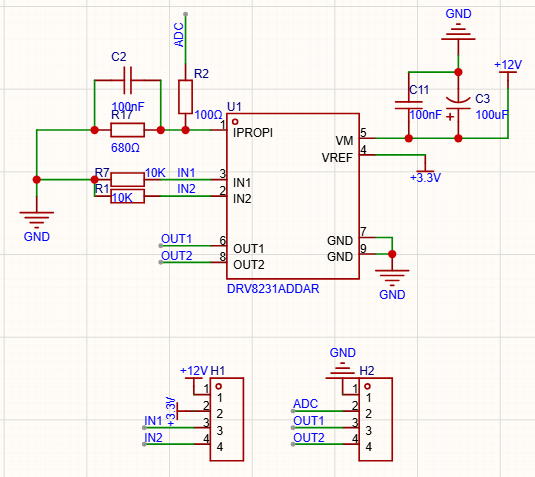
\includegraphics[width=0.72\textwidth]{sch_driver}
\caption*{DRV8231 单路电机驱动与电流采样电路；左右两路结构相同}
\end{figure}

\end{document}